\documentclass[main.tex]{subfiles}
\begin{document}

\chapter{Voorbeelden}
\label{cha:voorbeelden}

\section{Symbolen, strings en talen}
\label{sec:symbolen-strings-talen}

\begin{vb}
  Een letter, teken, of ander character op uw toetsenbord is een symbool.
  \begin{center}
  `a',\ `b',\ `c',...,\ `z',\ `A',\ `B',\ `C',...,\ `Z',\ `0',\ `1',\ `2',...,\ `8',\ `9',...,\ `.',\ `;',...
  \end{center}
  De equivalentierelatie gedefinieerd op deze symbolen is eenvoudigweg de gelijkheid.
\end{vb}

\begin{vb}
  De typeklasse \texttt{Eq a} van Haskell komt overeen met symbolen.
  De equivalentierelatie is dan de \texttt{(==) :: a -\textgreater\ a -\textgreater\ Bool} functie.
\end{vb}

\begin{vb}
  De staten van een eindige toestandsautomaat kunnen we zien als symbolen.
  Voor de equivalentierelatie zijn er dan een aantal mogelijkheden:
  \begin{itemize}
  \item Wanneer we de staten nummeren kunnen we de gelijkheid van het identificatienummer
  \item $f$-gelijkheid.\deref{de:f-gelijk}
  \item Het beeld onder een isomorfisme tussen automaten.
  \end{itemize}
\end{vb}

\begin{vb}
  Zelfs volledige automaten kunnen we zien als symbolen.
  Als equivalentierelatie kunnen we dan de equivalentie of isomorfismen beschouwen.
\end{vb}

\begin{vb}
  Woorden zijn strings met als symbolen eenvoudige letters.
\end{vb}

\begin{vb}
  Paden in automaten kunnen we beschouwen als strings met staten als symbolen.
\end{vb}

\begin{vb}
  Zelfs een opeenvolging van overgangen van equivalente automaten kunnen we zien als een string.
  Hier kiezen we dan de equivalentie van die automaten als equivalentierelatie.
\end{vb}

\begin{vb}
  Alle woorden in de nederlandse taal vormen een ... taal (duh).
\end{vb}

\begin{vb}
  Alle even getallen vormen een taal met cijfers als symbolen.
\end{vb}

\begin{vb}
  Alle reguliere expressies vormen een taal.
\end{vb}

\begin{vb}
  De verzameling van alle automaten vormt een taal.
\end{vb}

\begin{vb}
  De reguliere expressie $(a|b)c$ bepaalt de taal $\{ac, bc\}$
\end{vb}

\begin{vb}
  De reguliere expressie $(ab|c)^{*}d$ bepaalt de volgende taal:
  \[ \{d, abd, cd, ababd, abcd, cabd, ccd, \dotsc \}\]
\end{vb}

\section{Eindige Toestandsautomaten}
\label{sec:eind-toestandsautomaten}

\begin{vb}
  Zij $\{ 0 \}$ een alfabet $\Sigma$ en zijn $q_{s}$, $q'$ en $q_{f}$ staten, dan is het volgende $5$-tal een NFA:
  \[ \left(\left\{q_{s},q',q_{f}\right\},\left\{0\right\},\left\{\left((q_{s},0),\{q'\}\right),\left((q',0),\{q',q_{f}\}\right)\right\},q_{s},\left\{q_{f}\right\} \right) \]
  De figuur maakt dit duidelijker:
  \begin{figure}[H]
    \centering
    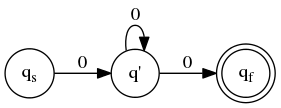
\includegraphics[width=0.3\textwidth]{assets/nfa-vb1.png}
    \caption{Een voorbeeld NFA}
    \label{fig:nfa-vb1}
  \end{figure}
\end{vb}

\begin{vb}
  Werking van bovenstaande nfa bij input string $00$:\\
  In stap $1$ kijken we naar het eerste symbool van $00$, een $0$.
  De overgangsfunctie $\delta$ zegt ons dat we met een $0$ in staat $q_{s}$ naar $q'$ kunnen gaan.
  \[ \delta(q_{s},0) = \left\{q'\right\} \]
  \begin{figure}[H]
    \centering
    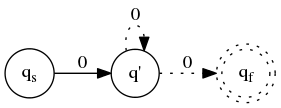
\includegraphics[width=0.3\textwidth]{assets/nfa-vb2.png}
    \caption{Stap 1}
    \label{fig:nfa-vb2}
  \end{figure}
  Het volgende symbool is opnieuw een $0$, maar nu bevindt de machine zich in staat $q'$.
  Vanuit $q'$, met een $0$ kan de automaat naar zowel $q'$ als $q_{f}$ gaan.
  Er zijn na deze stap geen symbolen meer over, de automaat stopt.
  \[ \delta(q',0) = \left\{q',q_{f}\right\} \]
  \begin{figure}[H]
    \centering
    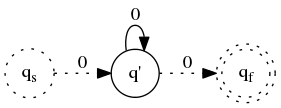
\includegraphics[width=0.3\textwidth]{assets/nfa-vb3.png}
    \caption{Stap 2.1}
    \label{fig:nfa-vb3}
  \end{figure}
  In het eerste geval eindigt de automaat in staat $q'$.
  \begin{figure}[H]
    \centering
    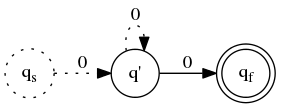
\includegraphics[width=0.3\textwidth]{assets/nfa-vb4.png}
    \caption{Stap 2.2}
    \label{fig:nfa-vb4}
  \end{figure}
  In het tweede geval eindigt de automaat in een accepterende toestand, en accepteert de automaat de string bijgevolg.
  Omdat er een opeenvolging $q_{s}q'q_{f}$ bestaat zodat de automaat de string aanvaardt, zeggen we dat de automaat de string aanvaardt.
\end{vb}

\TODO{GNFA uitvoeren}
\TODO{transitietabel}
\TODO{DFA naar NFA}
\TODO{DFA minimalisatie}
\TODO{encoderingen}

\end{document}

